\section{Introduction}

\subsection{Contexte}
\begin{frame}[t]{\mysubsectiontitle}
	Motivations
	\begin{itemize}
		\item La jurisprudence est analysée par les juristes pour comprendre l'application de la loi 
	    \item Difficultés de l'analyse manuelle
	    \begin{itemize}
	    	\item Existence d'un gros volume de décisions 
	    		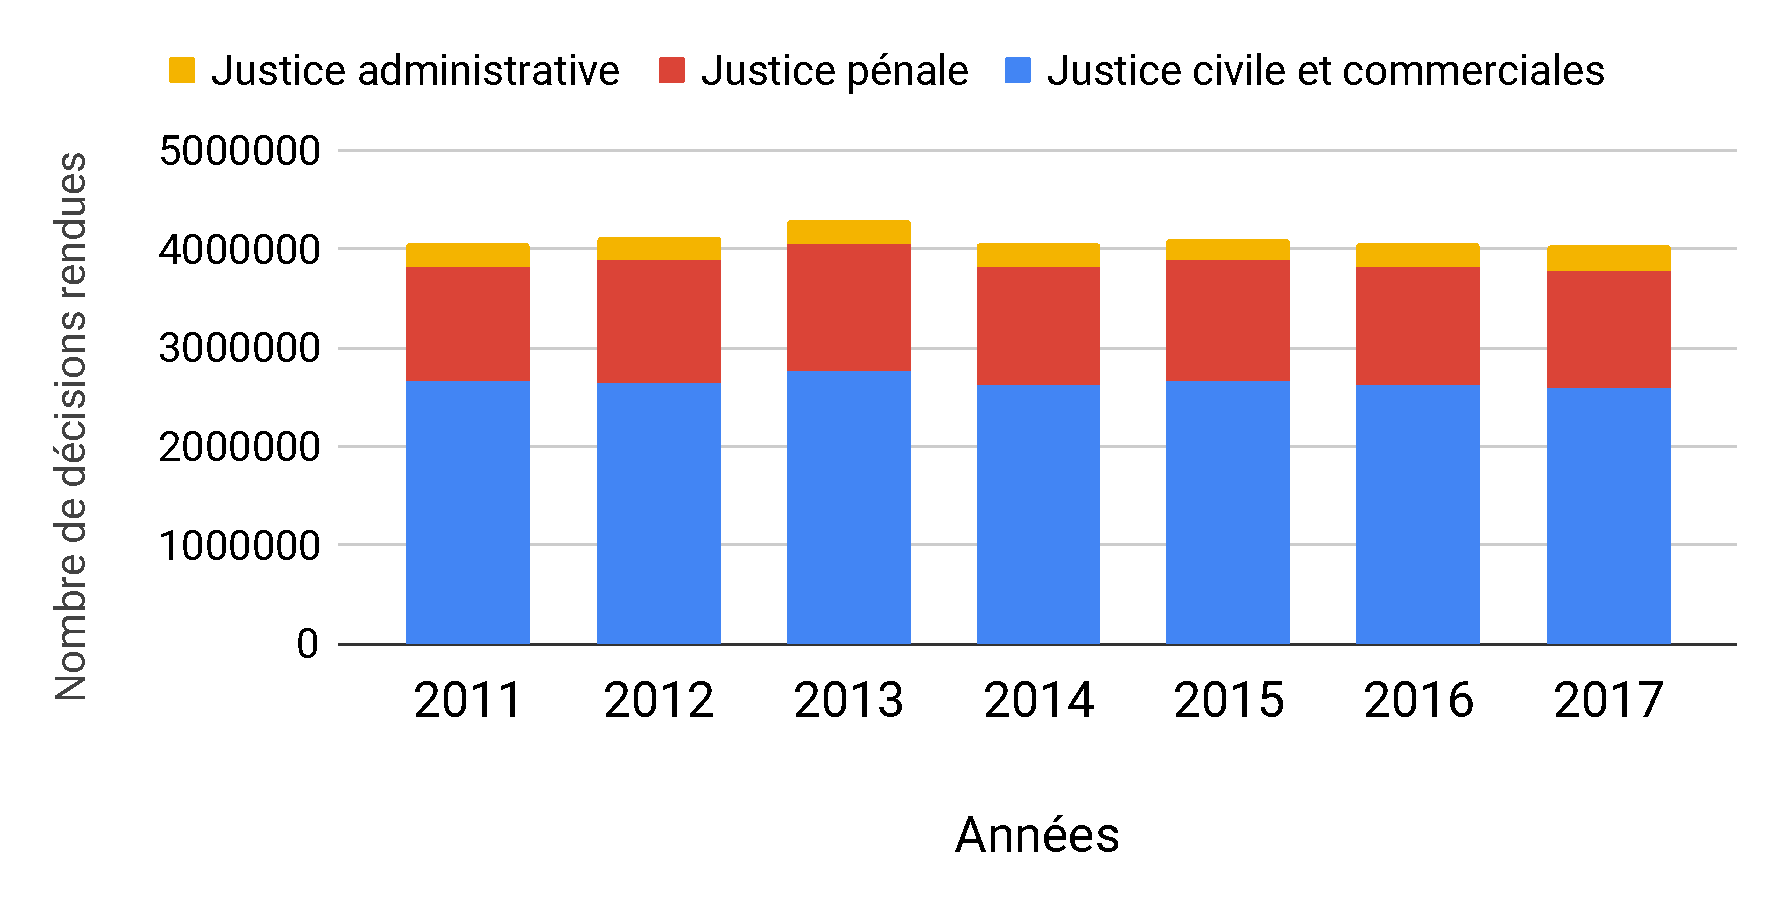
\includegraphics[width=0.6\textwidth]{chiffres-justice.pdf}   	
			\item Les moteurs de recherche juridique limitées : 
			\begin{itemize}
				\item Pas de critère de recherche sémantique (catégorie de demandes, type de faits, etc.)
				\item pas d'analyse synthétique de corpus
			\end{itemize}
	    \end{itemize}
	\end{itemize}
\end{frame}

%\subsection{État de l'art}
\begin{frame}[t]{\mysubsectiontitle}
	Activités en analyse automatique de décisions judiciaires	
	\begin{itemize}\scriptsize
		\item Extraction d'information dans les décisions
		\begin{itemize}  \scriptsize
			\item Entités juridiques \cite{Waltl2016lexia, andrew2018legalNerAndRelation}
			\item Faits \cite{wyner2010extractlegalelts, wyner2010casefactors, Shulayeva2017recognfactprincip}
			\item Définitions de concept juridiques \cite{Waltl2016lexia,waltl2017legaliegerman}
			\item Arguments \cite{moens2007NBvsMaxent4arguments}
		\end{itemize}
		\item Classification de décisions
		\begin{itemize} \scriptsize
			\item Prédiction des décisions de justice \cite{Ashley2009classifCases, Aletras2016predictDecisionECHR}
			\item Identification de la formation et la période \cite{Sulea2017predictareadecision,sulea2017legalEnsSVM}
			\item Identifier la sentence prononcée \cite{ma2018wmdchinesecase}
		\end{itemize}
		\item Similarité entre décisions 
		\begin{itemize}  \scriptsize
			\item Décisions qui citent les mêmes lois et précédents \cite{nair2018judgsimassorule}
			\item Similarité basée sur la question discutée et les faits sous-jacents  \cite{kumar2011judgmentsimilarity}
			\item Recherche d'affaires antérieures pertinentes  \cite{thenmozhi2017legalprecedretriev}
			\item Classification supervisée des décisions \cite{ma2018wmdchinesecase}
			\item Regroupement non-supervisé \cite{raghuveer2012legalclusteringLDA}
		\end{itemize}
	\end{itemize}
\end{frame}

\subsection{Objectif de la thèse}
\begin{frame}[c]{\mysubsectiontitle}
	Tâches et exemples d'applications
		
	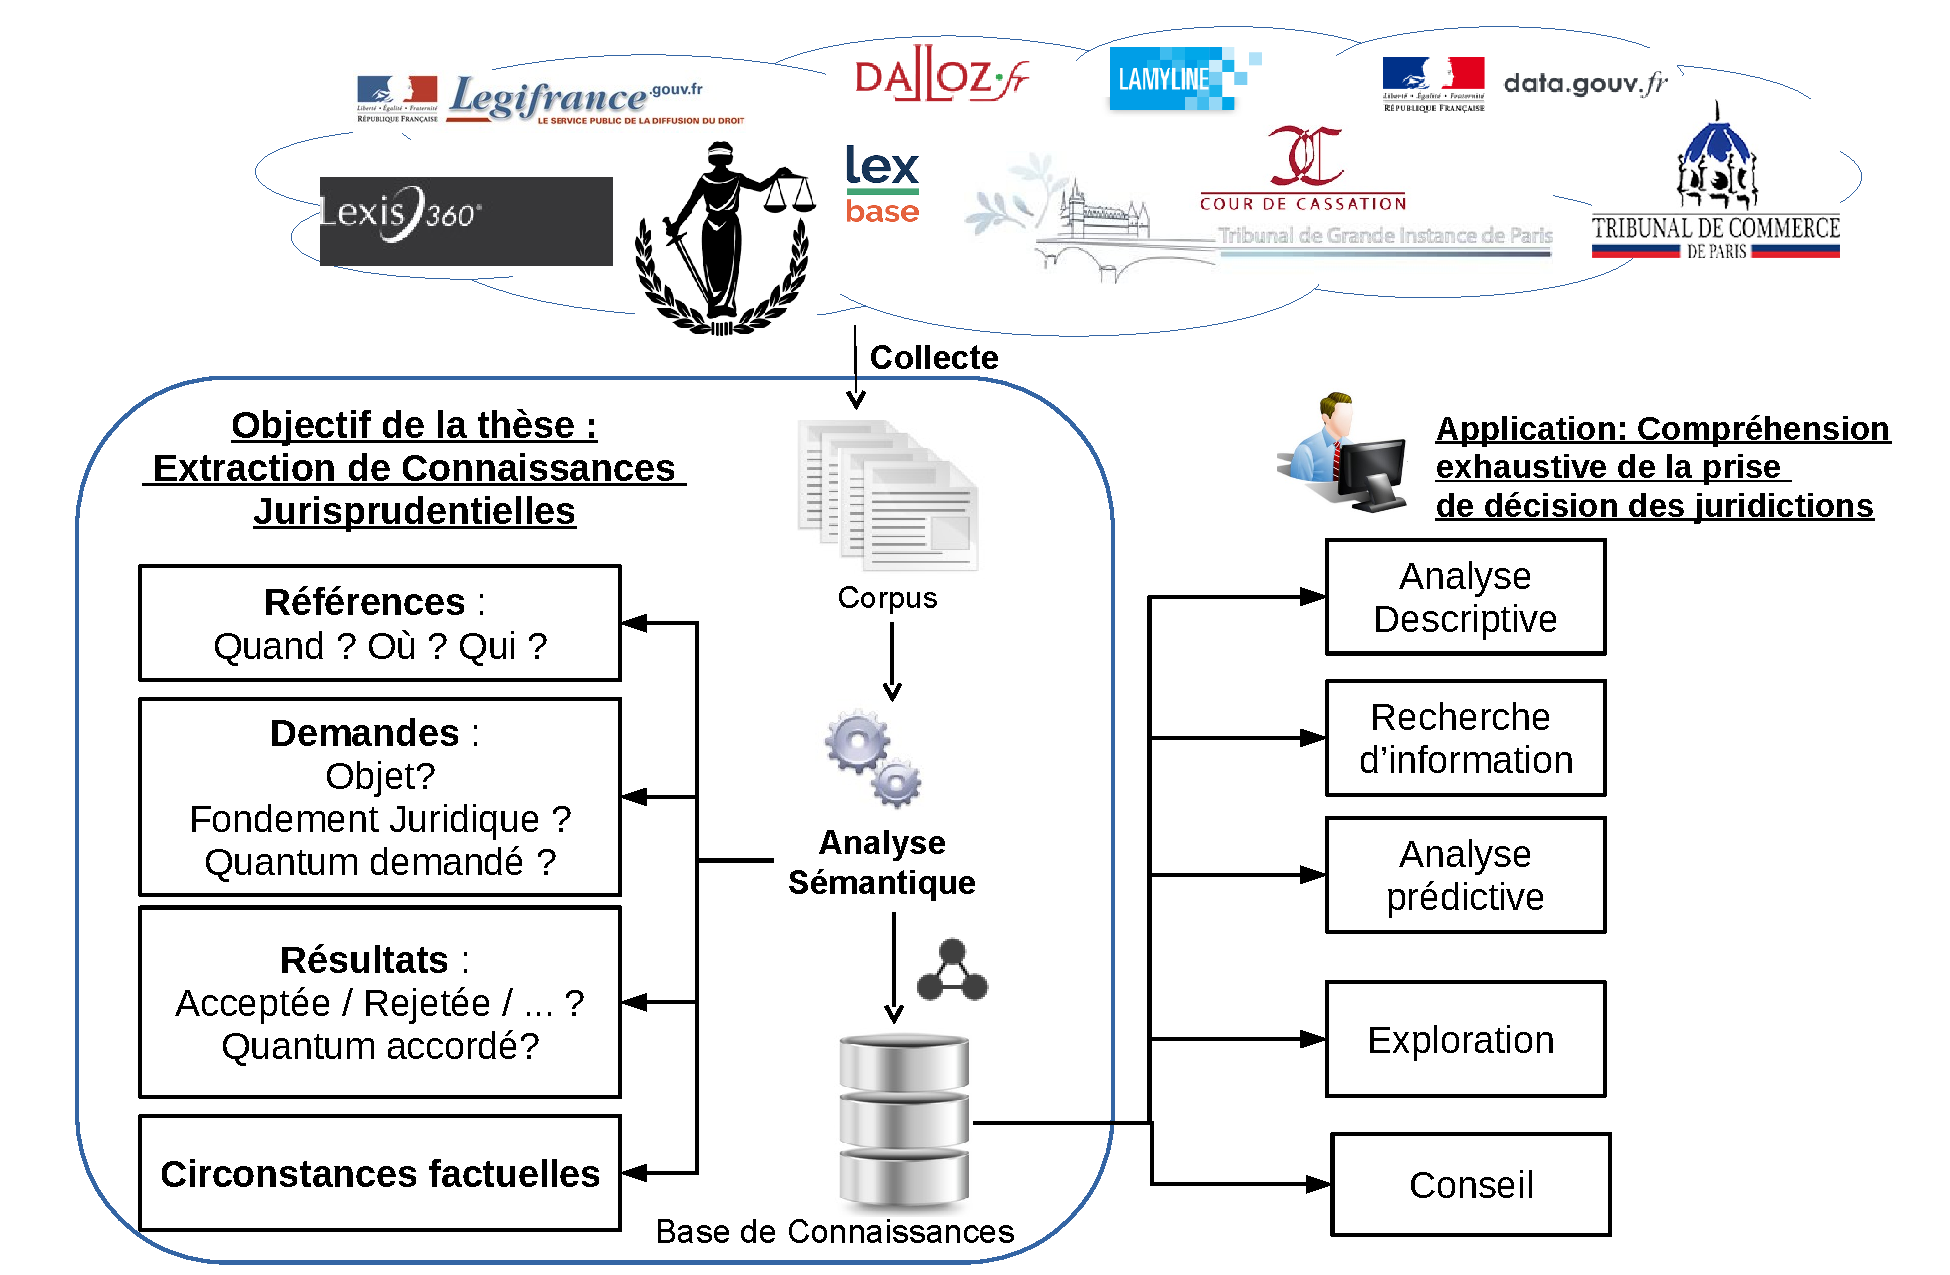
\includegraphics[width=\textwidth]{Objectif_these.pdf}	
\end{frame}

\begin{frame}[c]{\mysubsectiontitle}	
	Formulation en analyse de données textuelles	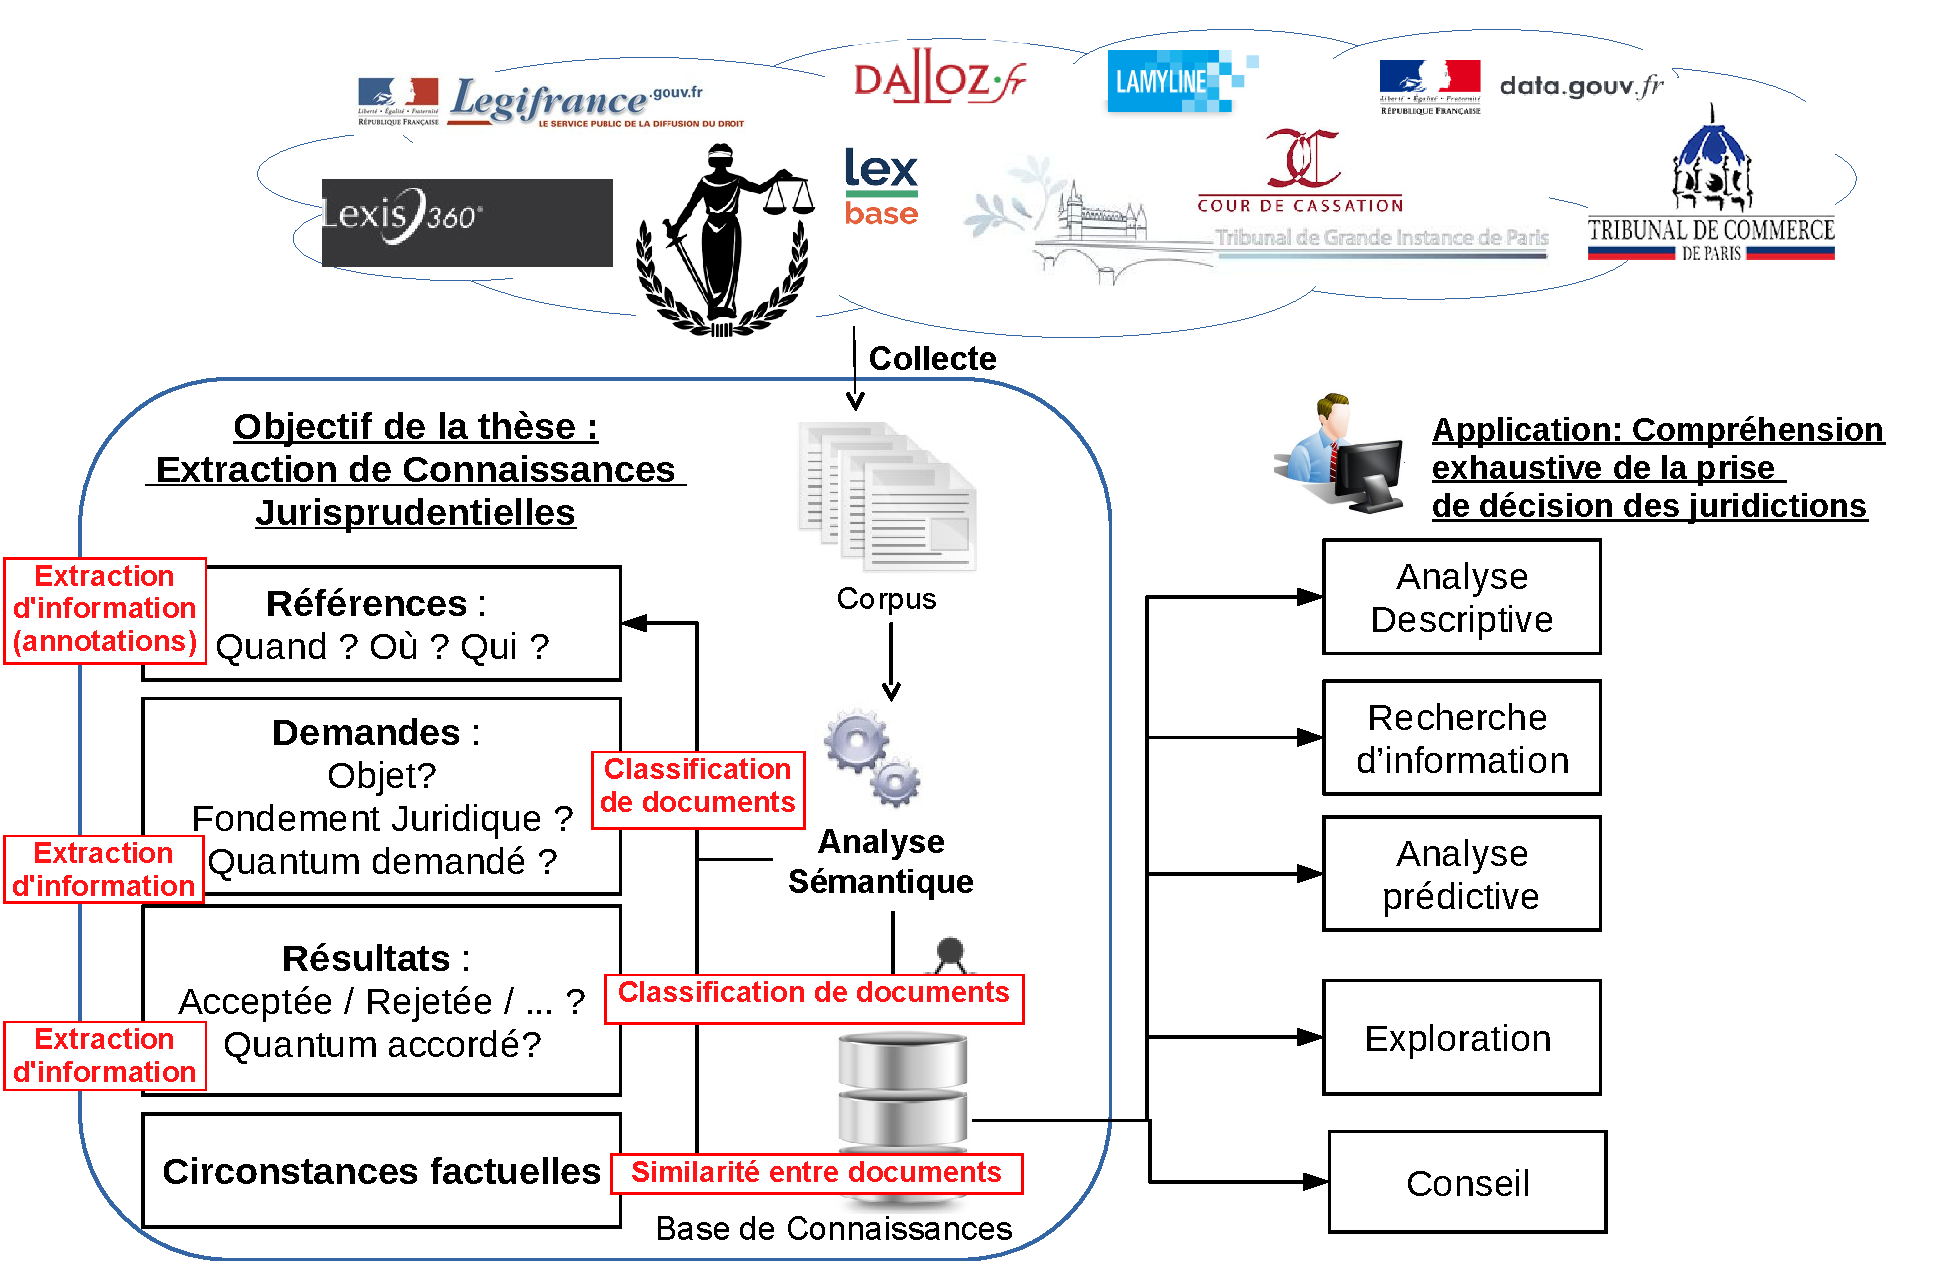
\includegraphics[width=\textwidth]{Objectif_these-problemes2.pdf}		
\end{frame}
